\begin{frame}{Features}
\centering
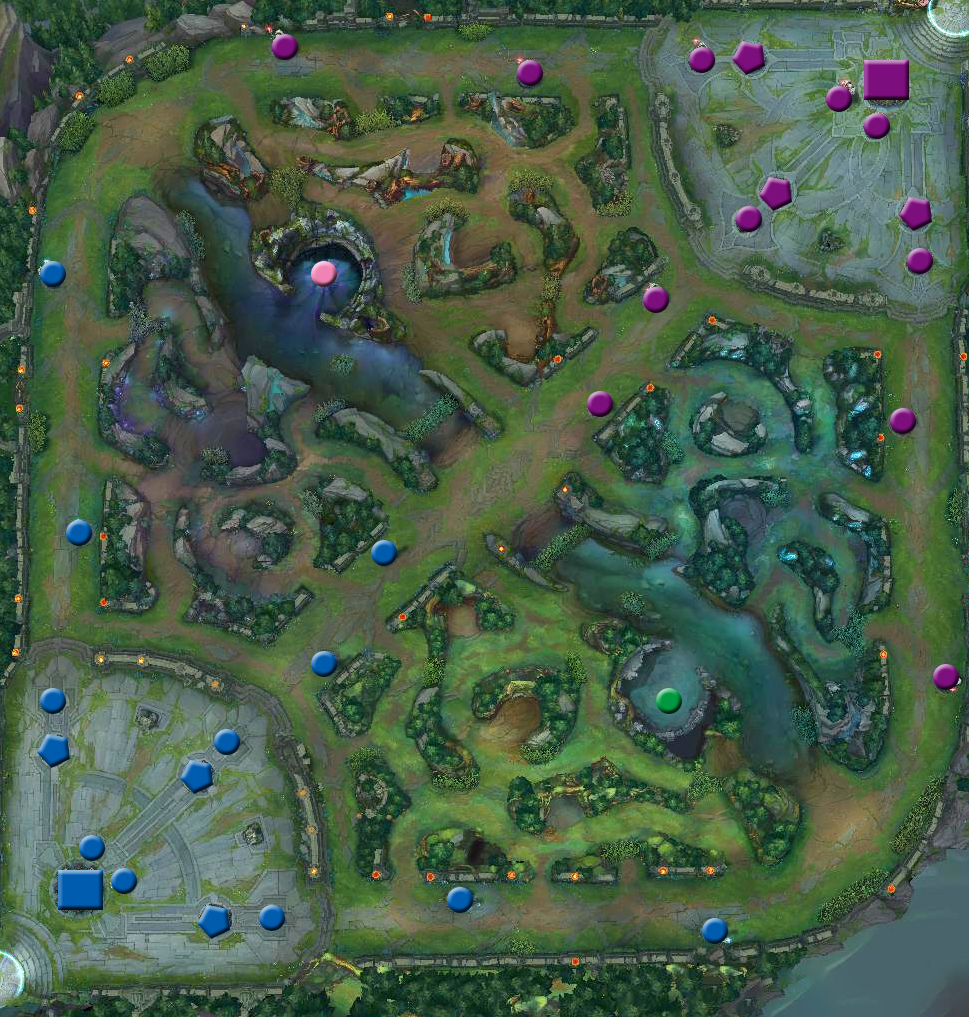
\includegraphics[scale=0.2]{img/kent/lolmap.jpg}
\end{frame}

\begin{frame}{Features}
\centering
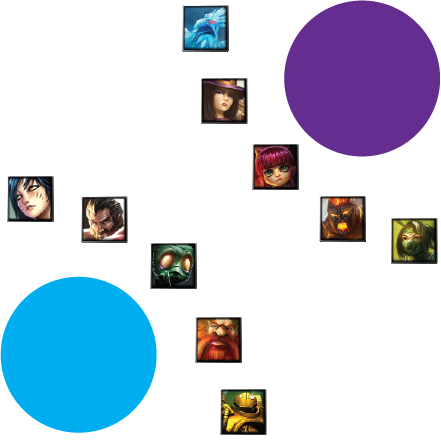
\includegraphics[scale=0.35]{img/kent/1.png}\\
\vspace{8pt}
$P(Winner = \textcolor{blue}{\text{blue}}) = \alpha$
\end{frame}

\begin{frame}{Features}
\centering
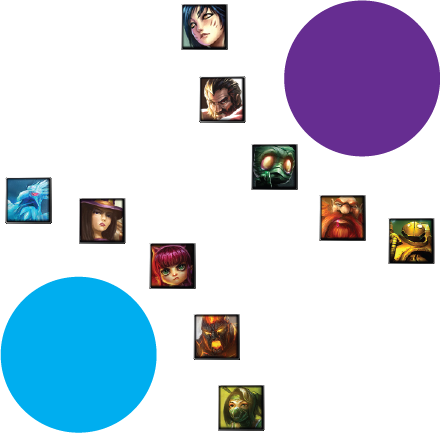
\includegraphics[scale=0.35]{img/kent/2.png}\\
\vspace{8pt}
$P(Winner = \textcolor{purple}{\text{purple}}) = \alpha ?$
\end{frame}

\begin{frame}{Features}
\centering
\textcolor{blue}{Team blue} (won)

\includegraphics[scale=0.4]{img/kent/pickblue.png}\\
\vspace{20pt}
\textcolor{purple}{Team purple} (lost)

\includegraphics[scale=0.4]{img/kent/pickpurple.png}\\
\end{frame}

\begin{frame}{Binary representation}
\centering
\textcolor{blue}{Team blue} (won) \hspace{40pt} \textcolor{purple}{Team purple} (lost)\\

\includegraphics[width=0.47\textwidth]{img/kent/pickblue.png}\hspace{2pt}%

\includegraphics[width=0.47\textwidth]{img/kent/pickpurple.png}\\
\vspace{18pt}
$x =$\\
\hspace{2pt} $(\textcolor{blue}{0,\;1,\;0,\;0,\;1,\;1,\;0,\;1,\;1,\;0,\;...},\textcolor{purple}{1,\;0,\;1,\;1,\;1,\;0,\;0,\;0,\;1,\;0,...})$\\
\vspace{18pt}
$y = \textcolor{blue}{\text{true}}$
\end{frame}

\begin{frame}{Mirrored binary representation}
\centering
\textcolor{blue}{Team blue} (won) \hspace{40pt} \textcolor{purple}{Team purple} (lost)\\

\includegraphics[width=0.47\textwidth]{img/kent/pickblue.png}\hspace{2pt}%

\includegraphics[width=0.47\textwidth]{img/kent/pickpurple.png}\\
\vspace{18pt}
$x =$\\
\hspace{2pt} $(\textcolor{blue}{0,\;1,\;0,\;0,\;1,\;1,\;0,\;1,\;1,\;0,\;...},\textcolor{purple}{1,\;0,\;1,\;1,\;1,\;0,\;0,\;0,\;1,\;0,...})$\\
$y = \textcolor{blue}{\text{true}}$\\
\vspace{18pt}
$x' =$\\
\hspace{2pt} $(\textcolor{purple}{0,\;1,\;0,\;0,\;1,\;1,\;0,\;1,\;1,\;0,\;...},\textcolor{blue}{1,\;0,\;1,\;1,\;1,\;0,\;0,\;0,\;1,\;0,...})$\\
$y' = \textcolor{purple}{\text{false}}$
\end{frame}

\begin{frame}{Compact binary representation}
\centering
\textcolor{blue}{Team blue} (won):\\
\hspace{20pt}
\includegraphics[width=0.47\textwidth]{img/kent/pickblue.png}\\
\vspace{8pt}
$x = (\textcolor{blue}{0,\;1,\;0,\;0,\;1,\;1,\;0,\;1,\;1,\;0,\;...})$\\
$y = \textcolor{blue}{\text{true}}$\\
\vspace{40pt}
\textcolor{purple}{Team purple} (lost):\\
\hspace{20pt}
\includegraphics[width=0.47\textwidth]{img/kent/pickpurple.png}\\
\vspace{8pt}
$x' = (\textcolor{purple}{1,\;0,\;1,\;1,\;1,\;0,\;0,\;0,\;1,\;0,\;...})$\\
$y' = \textcolor{purple}{\text{false}}$
\end{frame}

\begin{frame}{Ternary representation}
\centering
\textcolor{blue}{Team blue} (won)\\
\hspace{20pt}
\includegraphics[scale=0.31]{img/kent/pickblue.png}\\
\vspace{20pt}
\textcolor{purple}{Team purple} (lost)\\
\hspace{20pt}
\includegraphics[scale=0.31]{img/kent/pickpurple.png}\\
\vspace{20pt}
$x = (\textcolor{purple}{-1},\;\textcolor{blue}{1},\,\textcolor{purple}{-1},\textcolor{purple}{-1},\;0,\;\,\textcolor{blue}{1},\;\;0,\;\,\,\textcolor{blue}{1},\;\;0,\;\;0,\;\,...)$\\
$y = \textcolor{blue}{\text{true}}$\\
\end{frame}

\begin{frame}{Features}
\centering
Forcing symmetry:
\begin{itemize}
\item Good for a small training set
\item Worse or equal for a large training set
\end{itemize}

Best representation:
\begin{itemize}
\item Binary representation
\end{itemize}
\end{frame}

\begin{frame}{Features}
\centering
Not only single champions:
\begin{itemize}
\item Pairs of champions
\item Rank of players
\item Choice of runes
\item Choice of masteries
\item Lane of champions
\item ...
\end{itemize}

10 different types of features
\end{frame}


\begin{frame}{Features}
\centering
FeatureCreator:
\begin{itemize}
\item Introducing new features
\item Combining features
\end{itemize}
\end{frame}

\begin{frame}{Features}
Introducing a new type of feature:
\begin{itemize}
\item Initializer function: Provide the name of all possible features
\item Feature extractor function: Given a game object, identify the features present in that game
\end{itemize}
\end{frame}

\begin{frame}{Features}
Introducing feature $\phi_\text{SINGLE-CHAMPION}$
\begin{itemize}
\item Initializer function: 
	\begin{itemize}
	\item $\text{BLUE-Ahri},$
	\item $\text{BLUE-Akali}$
	\item ...
	\item $\text{BLUE-Zyra}$
	\item $\text{RED-Akali}$
	\item $\text{RED-Ahri}$
	\item ...
	\item $\text{RED-Zyra}$
	\end{itemize}
\item Feature extractor function:  
	\begin{itemize}
	\item Game object $\rightarrow \{\text{BLUE-Olaf}, \text{BLUE-Ryze}, \text{RED-Lulu}, ...\}$
	\end{itemize}
\end{itemize}
\end{frame}